% Figure 1 --- the framework's eight stages.
%
% Standalone source for figures/fig_pipeline.pdf. This figure was once
% inlined as a tikzpicture inside sections/method.tex, which meant the
% shipped PDF could not be regenerated from the repository without
% recompiling the whole manuscript --- the one figure in a paper about
% reproducibility that was not itself a regenerable artefact. It is now a
% committed PDF with its source beside it, like fig_share_ecdf.pdf.
%
% Regenerate (from paper/); -cd makes latexmk write the PDF next to the
% source, in figures/, rather than into the current directory:
%     latexmk -cd -pdf figures/fig_pipeline.tex
%
% The tikz body below is the single source of truth; method.tex includes
% the built PDF and no longer carries a copy of it.
\documentclass[border=2pt]{standalone}
\usepackage[T1]{fontenc}
\usepackage{tikz}
\usetikzlibrary{positioning,arrows.meta}
\begin{document}
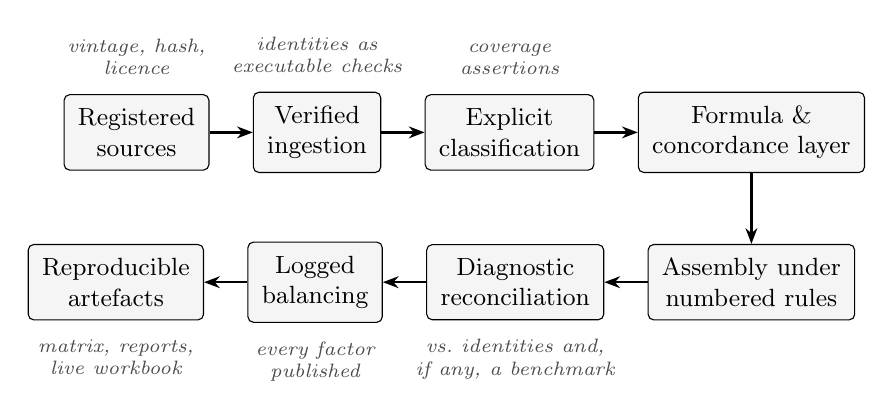
\begin{tikzpicture}[
  stage/.style={draw, rounded corners=2pt, align=center, font=\small,
                minimum height=2.2em, inner sep=5pt, fill=gray!8},
  note/.style={font=\scriptsize\itshape, text=gray!60!black, align=center},
  arr/.style={-{Stealth[length=2mm]}, thick}]
\node[stage] (s1) {Registered\\sources};
\node[stage, right=0.55cm of s1] (s2) {Verified\\ingestion};
\node[stage, right=0.55cm of s2] (s3) {Explicit\\classification};
\node[stage, right=0.55cm of s3] (s4) {Formula \&\\concordance layer};
\node[stage, below=0.9cm of s4] (s5) {Assembly under\\numbered rules};
\node[stage, left=0.55cm of s5] (s6) {Diagnostic\\reconciliation};
\node[stage, left=0.55cm of s6] (s7) {Logged\\balancing};
\node[stage, left=0.55cm of s7] (s8) {Reproducible\\artefacts};
\draw[arr] (s1) -- (s2); \draw[arr] (s2) -- (s3);
\draw[arr] (s3) -- (s4); \draw[arr] (s4) -- (s5);
\draw[arr] (s5) -- (s6); \draw[arr] (s6) -- (s7); \draw[arr] (s7) -- (s8);
\node[note, above=0.12cm of s1] {vintage, hash,\\licence};
\node[note, above=0.12cm of s2] {identities as\\executable checks};
\node[note, above=0.12cm of s3] {coverage\\assertions};
\node[note, below=0.12cm of s6] {vs.\ identities and,\\if any, a benchmark};
\node[note, below=0.12cm of s7] {every factor\\published};
\node[note, below=0.12cm of s8] {matrix, reports,\\live workbook};
\end{tikzpicture}
\end{document}
